\begin{figure}[ht]
\begin{center}
 \begin{ccTexOnly}
   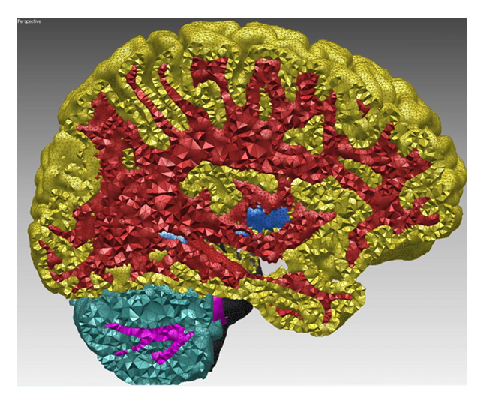
\includegraphics[height=9cm]{Mesh_3/pictures/multilabel_mesher}
 \end{ccTexOnly}
 \begin{ccHtmlOnly}
   <img border="0" src="./pictures/multilabel_mesher.jpg"><br/>
 \end{ccHtmlOnly}
 \caption{Cut-view of a multi-domain 3D mesh generated from a segmented image.}
  \label{figure:multilabel_mesher}
\end{center}
\end{figure}

\section{Introduction}
\label{Mesh_3_section_intro}

This package is devoted to the generation of  isotropic tetrahedron
meshes discretizing 3D domains. The main entry points of this component are
two global  functions that respectively generate
and refine such meshes.
%The main component of this package is a function which 
%generates 3D  simplicial meshes.
The domain to be discretized may be
formed either by a single connected component
or by several
connected components. We refer to the domain as a multi-domain
when the different components need to be
 identified  as different subdomains.
The mesh generator generates at once a simplicial 
3D mesh which includes one submesh for each subdomain
and surface meshes which approximate the boundaries 
 of the domain and subdomains.


\subsubsection{Input domain}

More specifically, the domain to be discretized is assumed
 to be representable as a pure
3D complex. A 3D complex is a set of faces with dimension
0 (vertices), 1 (edges), 2 (facets) and 3 (cells) such that
all faces are pairwise interior disjoint, 
and the boundary of each face of the complex is the union of faces
of the complex.
The 3D complex is pure, meaning that each face is included in a face of dimension 3,
so that the complex is entirely described as a set of 3D cells.
The set of faces with dimension lower or equal than 2 form a 2D
subcomplex. In the rest of the documentation, we will refer to the
input 3D complex as to the input domain.


Note that the input complex faces are not required to be linear. 
Facets, for instance, are typically smooth surface patches, 
or portion of surface meshes with boundaries.
The mesh generator provides at the same time
a 3D mesh discretizing each of the complex cells
and a surface mesh approximating the 2D complex 
that describes cell boundaries.
In its current state the mesh generator does not handle
sharp creases in the domain description. This does not mean  that 
the domain to be meshed  and its subdomains
are required to have smooth boundary surfaces.  The domain 
and  subdomains  boundaries  may be provided
 as smooth patches joined  along sharp edges.
However, currently, the mesh generator
 does  not take into account  the  edge description and hence
those edges are not  accurately  represented by a sequence of  mesh edges.


The mesh generator is able to handle
multiple junctions where three or more subdomains meet.
Consequently  the generated surface mesh may be non-manifold
as a whole, even if each  submesh approximating the boundary of a subdomain
is manifold.




The domain is input to the mesh generation function,
as a class 
devised to  answer queries about the domain as well as its subdomains.
Mainly, this class provides predicates which state
if  a given query point belongs 
to the domain or not, 
and in the affirmative, to which of the subdomains it belongs to.
Current implementation provides  classes to represent
domains defined by implicit functions, polyhedral domains
and domain defined through 3D labeled images.

% The resulting mesh is output as a subcomplex of a 3D triangulation,
% in the form of a class providing various output iterators
% on mesh elements.

\subsubsection{Output mesh}
\label{introsec:param}

The resulting mesh is output as a subcomplex of a 3D triangulation,
in a class  providing various iterators
on mesh elements. The 3D triangulation provides an approximation of the
domain, subdomains and their boundaries, according to the restricted
Delaunay triangulation paradigm. This means that the domain
(resp. each subdomain) is approximated by the union of  the tetrahedral cells
 whose circumcenters are located inside the domain
(resp. inside the subdomain). 
Each surface patch of the domain or subdomains boundary is approximated
by the union of   the Delaunay facets whose dual Voronoi edges intersect the surface patch.
Such facets are called in the following {\em surface facets} or {\em boundary facets}. 

The mesh generation algorithm is a Delaunay refinement process
followed by an optimization  phase, which is currently implemented
using the  sliver exudation approach~\cite{cgal:cdeft-slive-00}.
The   Delaunay refinement process is driven by criteria
concerning either the mesh cells 
or the surface facets.
%i.e., the facets of the mesh whose role is to approximate surface patches.
The refinement process terminates when there are
no more mesh cells or  surface facets violating the user-specified criteria.
The Delaunay refinement eliminates all kind of 
 quasi degenerate tetrahedra except slivers.
At the end of the refinement process,
some sliver shaped tetrahedra may occur in the mesh.
The optimization phase aims at eliminating slivers.




The criteria can  be tuned  to achieve the user needs with respect to
the size of mesh elements, the accuracy of boundary approximation
and topological conditions.
The default criteria  for surface facets are governed by the three following
parameters:
% \subsection{Parameters}
% \label{introsec:param}
%
% Some parameters are given to the refinment process to customize
% the generated mesh. Actually, each parameter correspond to a criteria
% that must be fullfilled by either each surface facet (if it is a
% \emph{surface facet parameter}) or each tetrahedron (if it is a
% \emph{cell parameter}). The mesh generation process ends when there is
% no more \emph{bad facet} or \emph{bad cell} given these criteria.
%
% In this package, we provide the following criteria. Note that each criteria may be
% deactivated by setting it to $0$.
%
%\subsubsection{Surface facet Parameters}
\begin{itemize}
\item \emph{the angular bound:} This parameter controls the shape of  
  surface facets. Actually, it is a lower bound for the angle (in degree) of
   surface mesh facets. The termination  of the meshing process is
garanted  if the angular bound is at most 30
  degrees. 
\item \emph{the radius bound:}  This parameter controls the size (edge
  length) of surface facets. Actually, each surface facet has 
a surface Delaunay ball which is a ball circumscribing the surface facet and
  centered on the surface patch.
 The radius bound is an upper 
  bound on the radii of surface Delaunay balls.
 \item \emph{the distance bound:}  This parameter controls the approximation error of the surface.
 Actually, it is an upper bound for the distance between the circumcenter
 of a surface facet and the center of a surface Delaunay ball of this facet.
\end{itemize}

%\subsubsection{Cell Parameters}
The default criteria for mesh cells are governed by two parameters:
\begin{itemize}
\item \emph{the radius-edge bound:}   This parameter controls the
  shape of mesh cells (but can't filter slivers, as we discuss earlier).
 Actually, it is an upper bound for the ratio
 between the circumradius of a 
   mesh tetrahedron and its shortest edge.
\item \emph{the radius bound:}  This parameter controls the size (edge length) of 
  mesh cells. Actually, it is an upper bound on the circumradii of the
 mesh tetrahedra.
\end{itemize}

Figure~\ref{figure:parameters} shows how the mesh generation process
behaves with respect to these parameters.

\begin{figure}[ht]
\begin{center}
 \begin{ccTexOnly}
   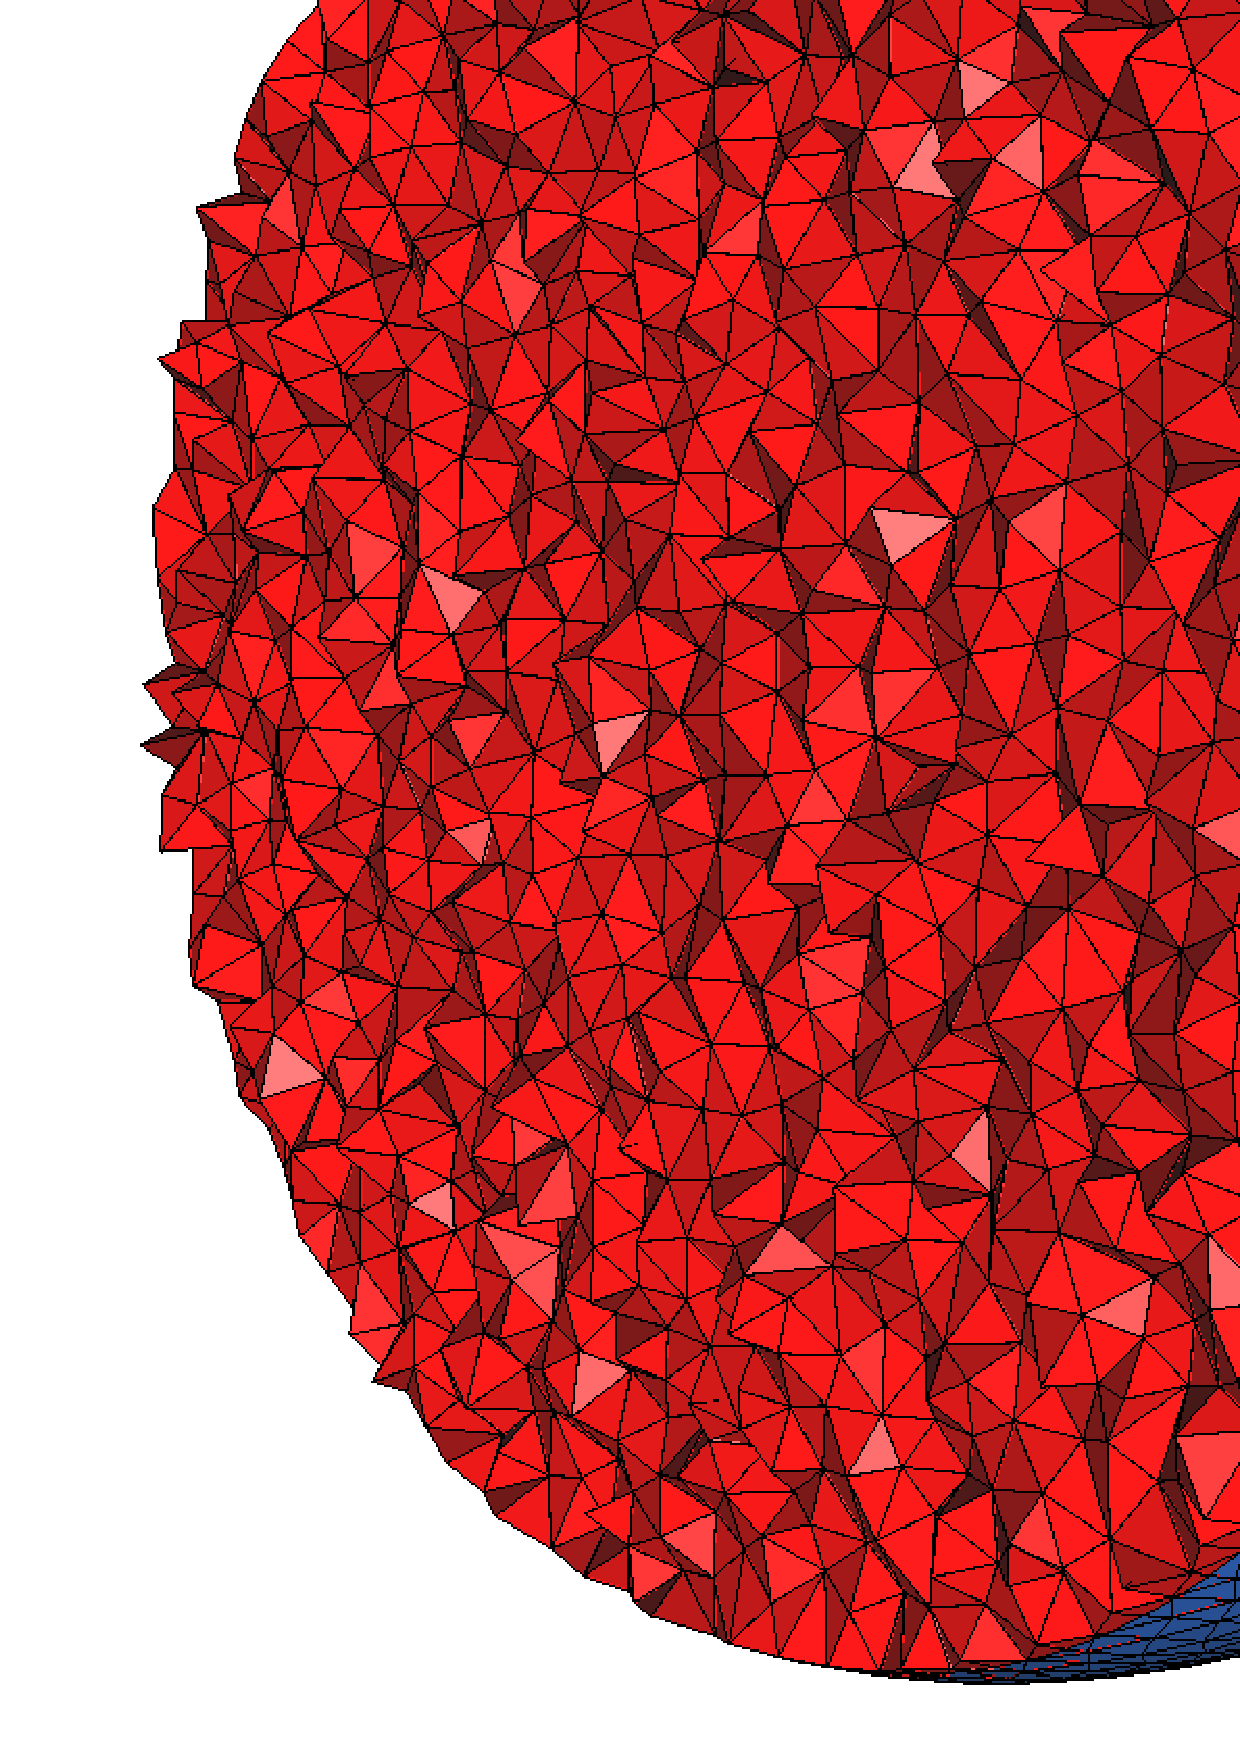
\includegraphics[height=5cm]{Mesh_3/pictures/implicit_domain}

   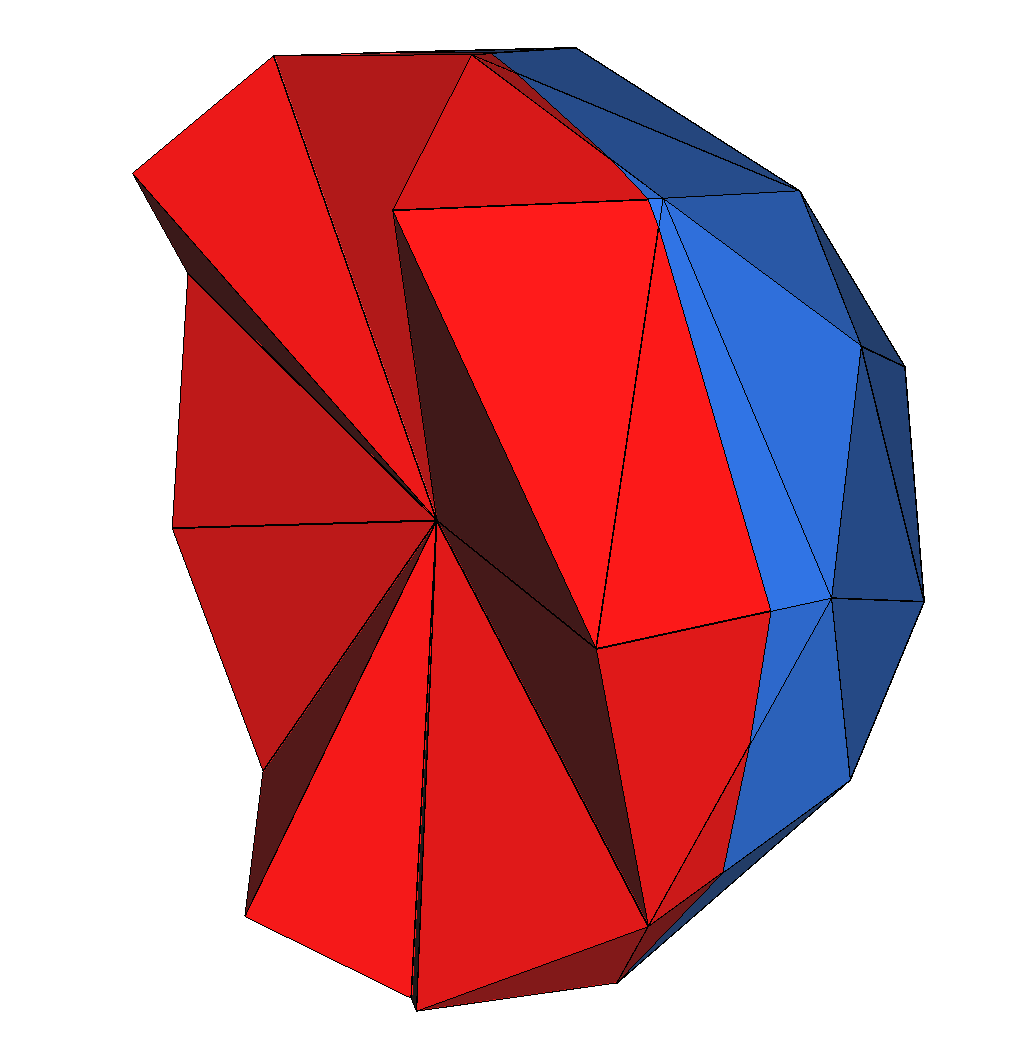
\includegraphics[height=5cm]{Mesh_3/pictures/implicit_domain_3}
   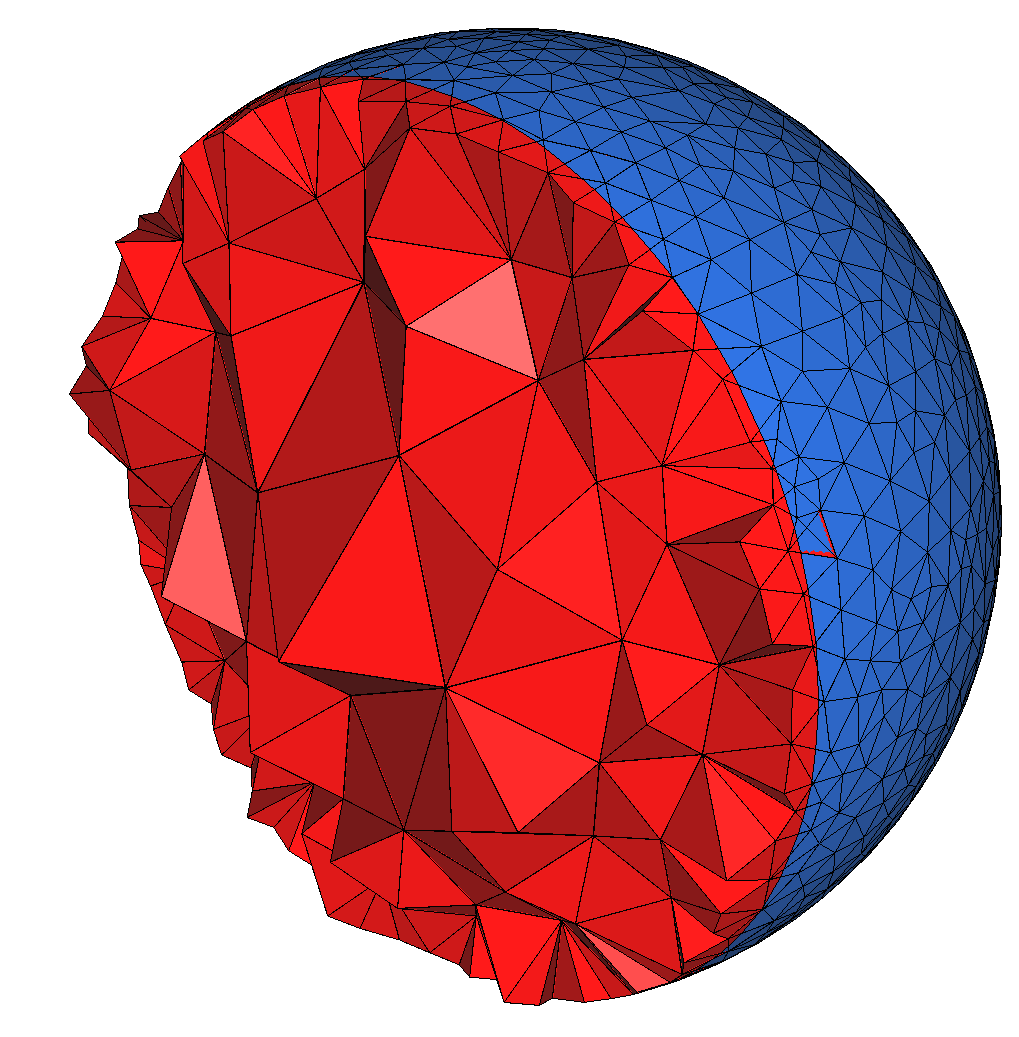
\includegraphics[height=5cm]{Mesh_3/pictures/implicit_domain_4}
   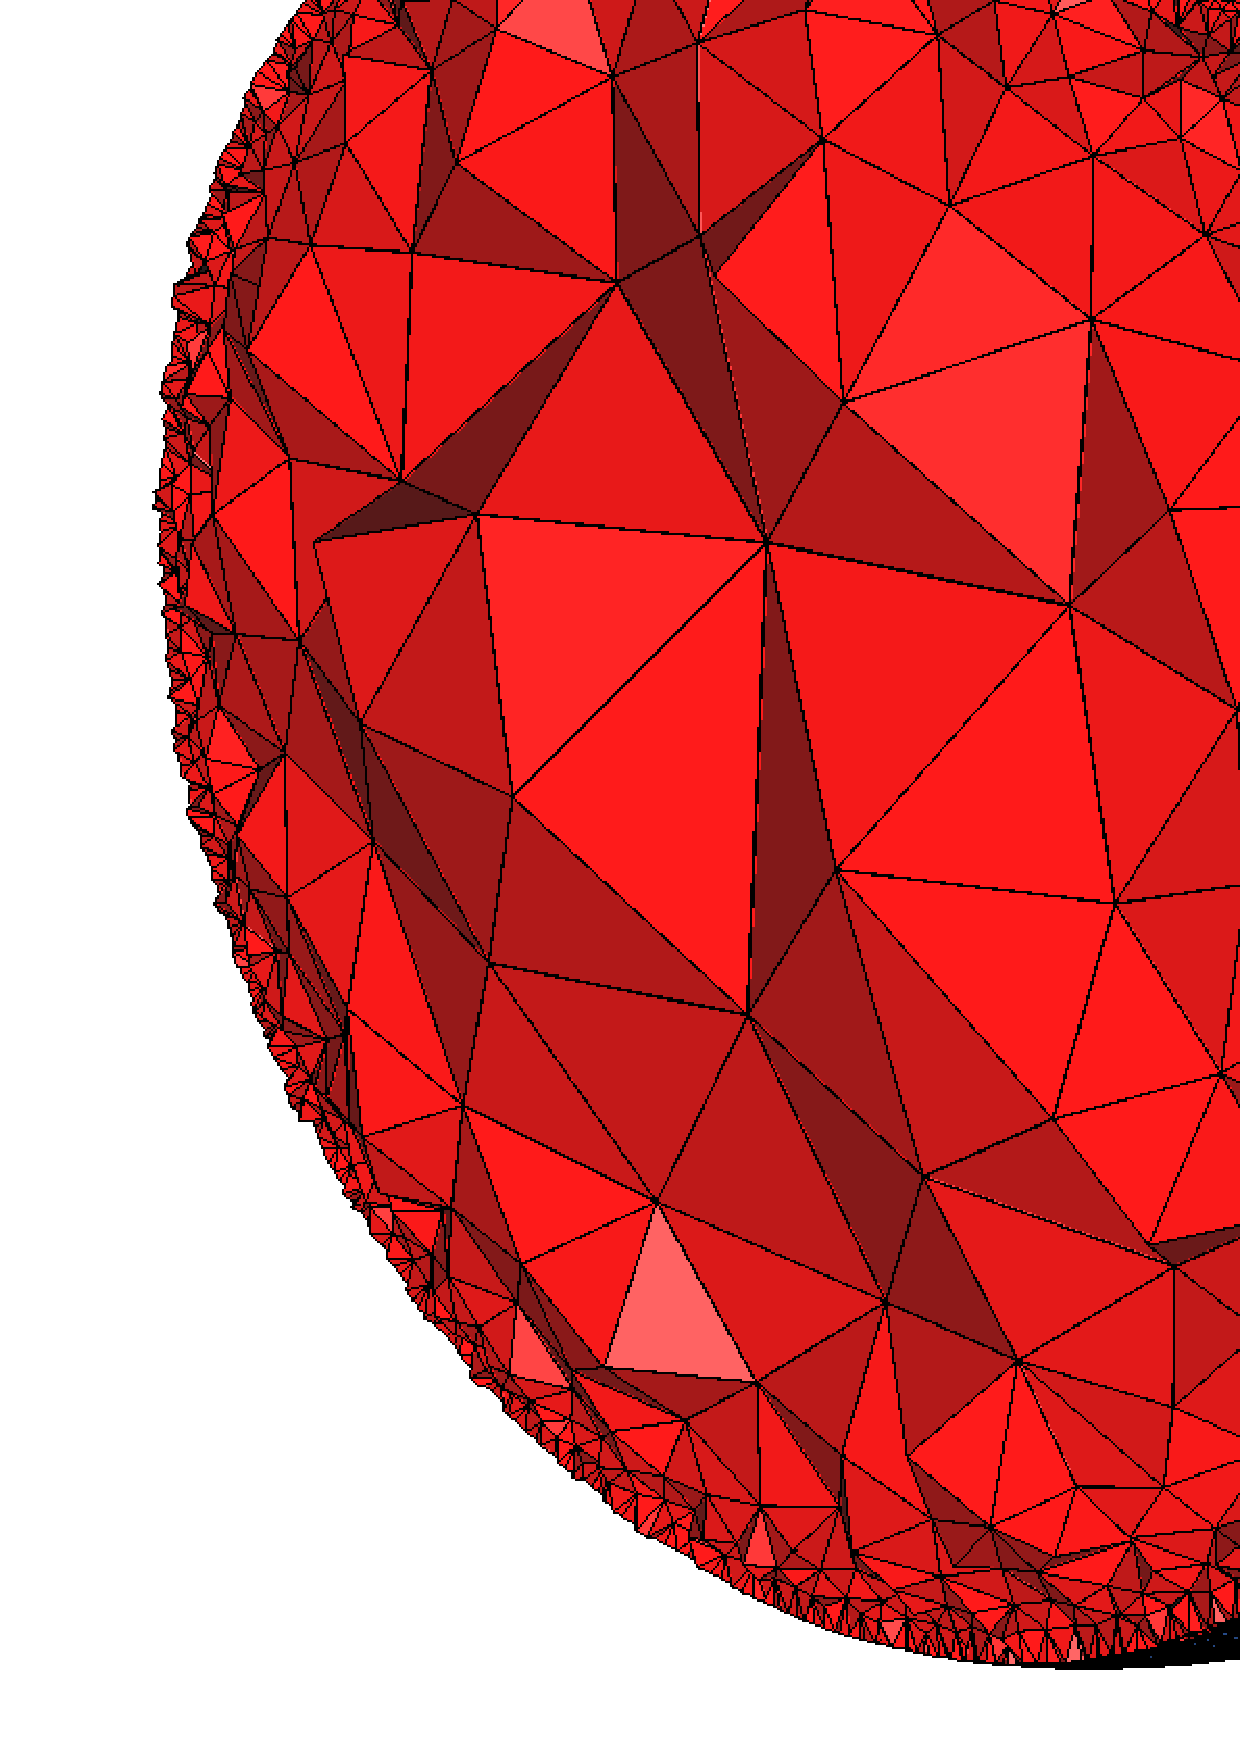
\includegraphics[height=5cm]{Mesh_3/pictures/implicit_domain_5}
 \end{ccTexOnly}
 \begin{ccHtmlOnly}
   <img border="0" height="250px" src="./pictures/implicit_domain.jpg"><br/>
   <img border="0" height="250px" src="./pictures/implicit_domain_3.jpg">
   <img border="0" height="250px" src="./pictures/implicit_domain_4.jpg">
   <img border="0" height="250px" src="./pictures/implicit_domain_5.jpg"><br/>
 \end{ccHtmlOnly}
 \caption{Top : the mesh  is obtained using the parameters $(25,0.15,0.05)$ for the angular bound,
radius bound and distance bound of  surface facets
and 
$(4,0.2)$ for  the radius-edge bound and radius  bound of mesh cells. The result is a  uniform mesh which contain tetrahedra
of about the same size. 
Bottom  left :
the mesh  is obtained by releaxing the \emph{ size bound} of tetrahedra
and facets.
 The result is a small coarse mesh. 
Bottom middle : the mesh  is obtained from the previous one  by tightening the \emph{distance bound} 
of surface facets to
$0.01$. The result is then a graded 3D mesh with a dense surface mesh
achieving a precise approximation. 
Bottom right :
the mesh  is obtained from the previous one  by fixing \emph{radius bound} of surface facets to
to $0.01$. The surface mesh is then denser to achieve the size bound.}
  \label{figure:parameters}
\end{center}
\end{figure}



\section{Interface}
\label{Mesh_3_section_interface}

A 3D mesh generation  process is called through a call
 to   one of the two following functions:
 
\ccGlobalFunction{
  template <class C3T3,
  class MeshDomain,
  class MeshCriteria>
  C3T3 make_mesh_3(MeshDomain domain, MeshCriteria criteria);}{}

\ccGlobalFunction{
  template <class C3T3,
  class MeshDomain,
  class MeshCriteria>
  void refine_mesh_3(C3T3& c3t3,
                     MeshDomain domain,
                     MeshCriteria criteria);}{}

The function \ccc{make_mesh_3} generates from scratch a mesh
of the input domain, while
the function \ccc{refine_mesh_3} refines
an existing mesh of the input domain.

The template parameter \ccc{C3T3} is required to be a model of
the concept 
\ccc{MeshComplex_3InTriangulation_3}, a data structure devised to
represent a three dimensional complex embedded in a 3D
triangulation. In both functions,  an instance  of type \ccc{C3T3} is used to maintain the current
approximating simplicial mesh of the domain and subdomains
and to represent the final  3D mesh at the end
of the procedure.
The type \ccc{C3T3} is   required to provide a nested type
\ccc{C3T3::Triangulation_3} for the 3D triangulation
embedding the mesh. This triangulation is required to be a regular
triangulation.
 The vertex and cell base classes of the
triangulation \ccc{C3T3::Triangulation_3} are required to be respectively  models of the
concepts \ccc{MeshVertexBase_3} and \ccc{MeshCellBase_3}.

The template parameter \ccc{MeshDomain} is required to be a model of
the concept  \ccc{MeshDomain_3}. The argument \ccc{mesh_domain} of type
\ccc{MeshDomain}
 is the sole link through which the domain
to be discretized is known  by the mesh generation algorithm. 
The concept \ccc{MeshDomain_3} is similar to the concept \ccc{SurfaceMeshTraits} 
defined by the surface mesh generation package.
This concept  provides, among others,
  member functions to test whether or not
a query segment intersects boundary surfaces,
and to compute an intersection point  in the affirmative.
The \ccc{MeshDomain_3} concept adds  member functions 
which given a query point tell whether the point lies
inside or outside the domain and in which subdomain the point lies
if inside.

% There are compatibility requirements between the template parameter 
% \ccc{C3T3} and \ccc{MeshDomain}.
% The nested types \ccc{MeshDomain::Subdomain_index},
% and \ccc{MeshDomain::Index} 
% have to be convertible respectively
% to the nested types \ccc{C3T3::Triangulation::Cell::Subdomain_index}
% and  \ccc{C3T3::Triangulation::Vertex::Index}.

The template parameter \ccc{MeshCriteria} must be a model of the concepts
\ccc{MeshCriteria_3}. 
The argument of
type \ccc{MeshCriteria} passed to the mesh generator specifies the
size and shape requirements for the tetrahedra in the mesh
and for the triangles in the boundary surface mesh. These criteria
form the rules which drive the refinement process.  At the end 
of the refinement process, every mesh element satisfy those criteria.
This may not be true anymore after the sliver removal phase although this
last phase is devised to only improve the mesh quality.




\section{Examples}
\label{Mesh_3_section_examples}


\subsection{Mesh Generation From an Implicit Domain}
The following code produces a 3D mesh for a monodomain whose boundary surface
is defined by an implicit
function. Figure~\ref{figure:implicit_domain} shows a cut view of the
resulting mesh.

\ccIncludeExampleCode{Mesh_3/mesh_implicit_sphere.cpp}

\begin{figure}[ht]
\begin{center}
 \begin{ccTexOnly}
   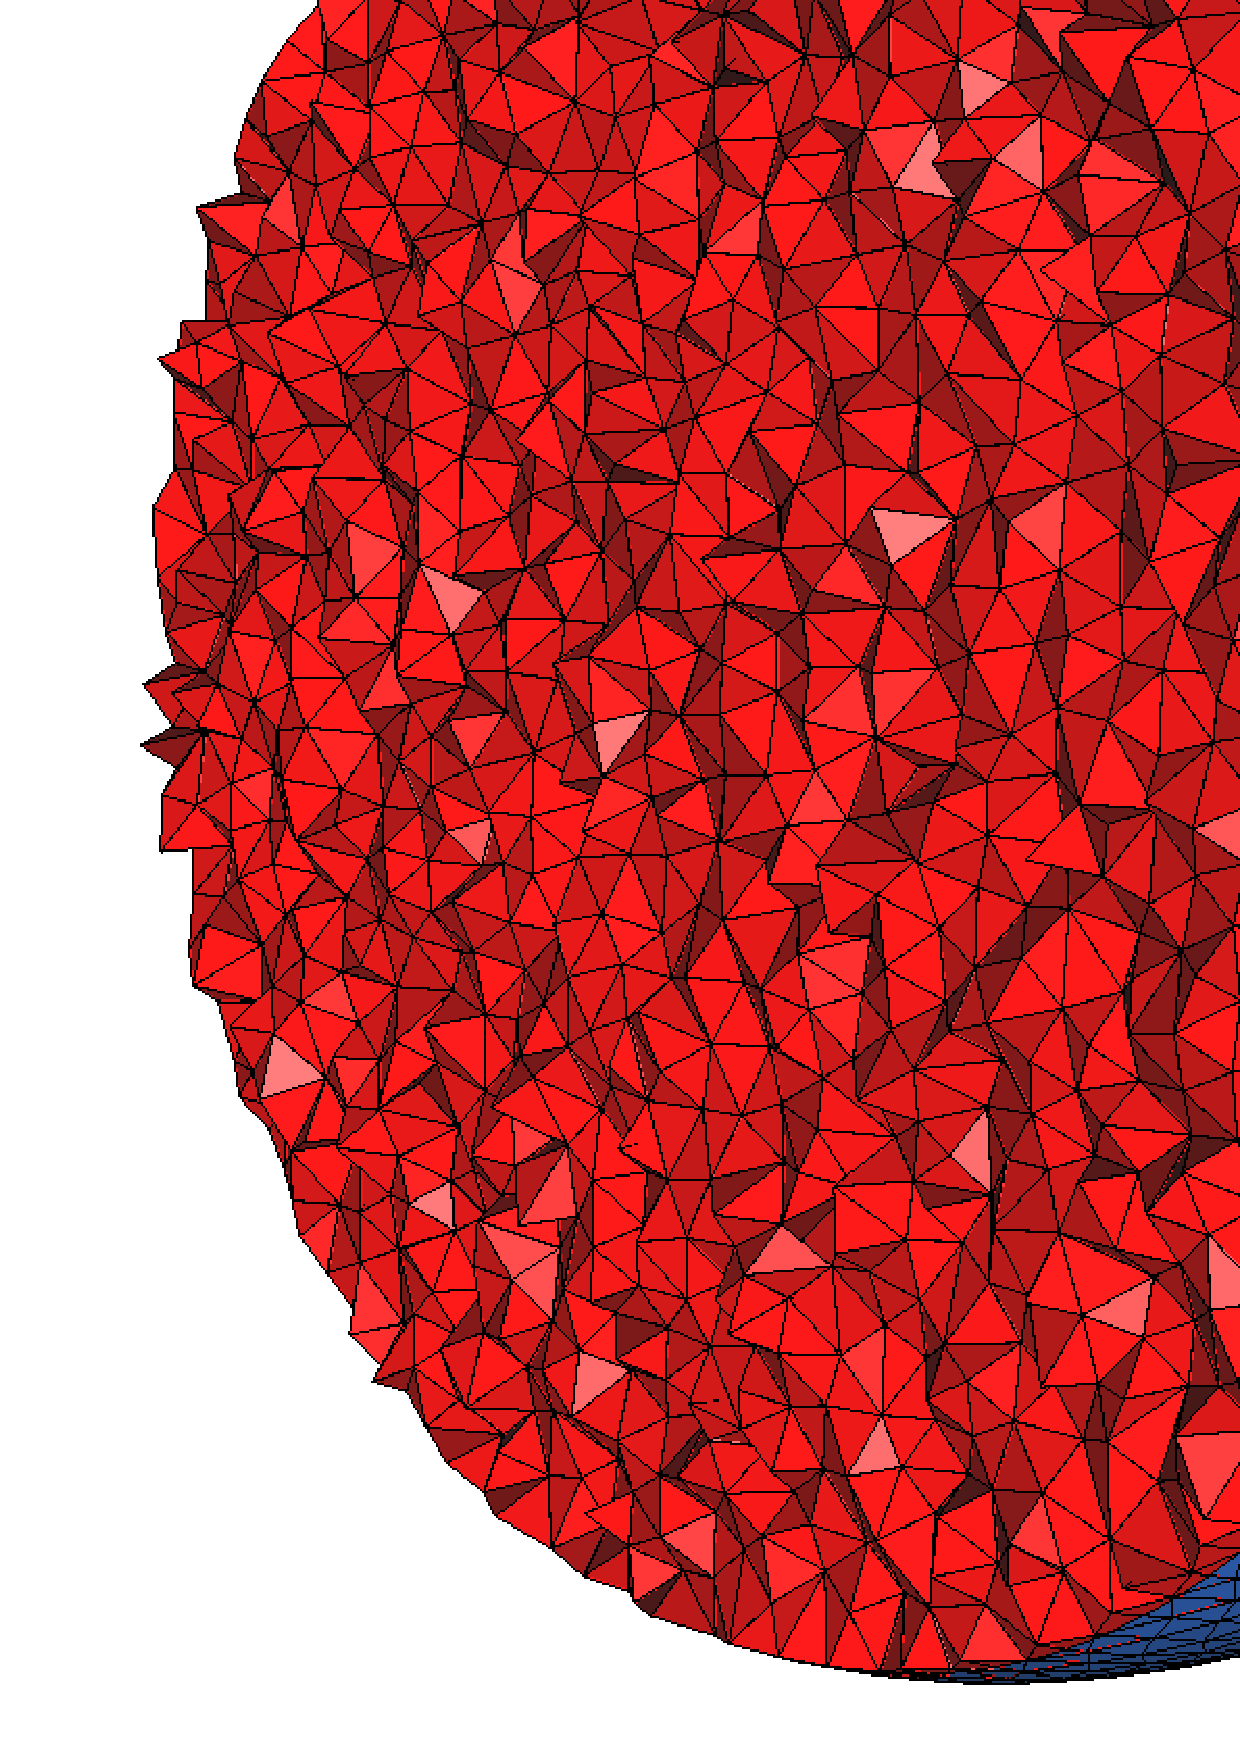
\includegraphics[height=6cm]{Mesh_3/pictures/implicit_domain}
 \end{ccTexOnly}
 \begin{ccHtmlOnly}
   <img border="0" src="./pictures/implicit_domain.jpg"><br/>
 \end{ccHtmlOnly}
 \caption{Cut-View of a 3D mesh produced from an implicit domain}
  \label{figure:implicit_domain}
\end{center}
\end{figure}


\subsection{Mesh Generation From a Polyhedral Domain}
\label{Mesh_3_subsection_examples_polyhedral}
The following code produces a 3D mesh for a monodomain
defined by polyhedral surfaces. Figure~\ref{figure:polyhedral_domain}
shows the resulting mesh.

\ccIncludeExampleCode{Mesh_3/mesh_polyhedral_domain.cpp}

\begin{figure}[ht]
\begin{center}
 \begin{ccTexOnly}
   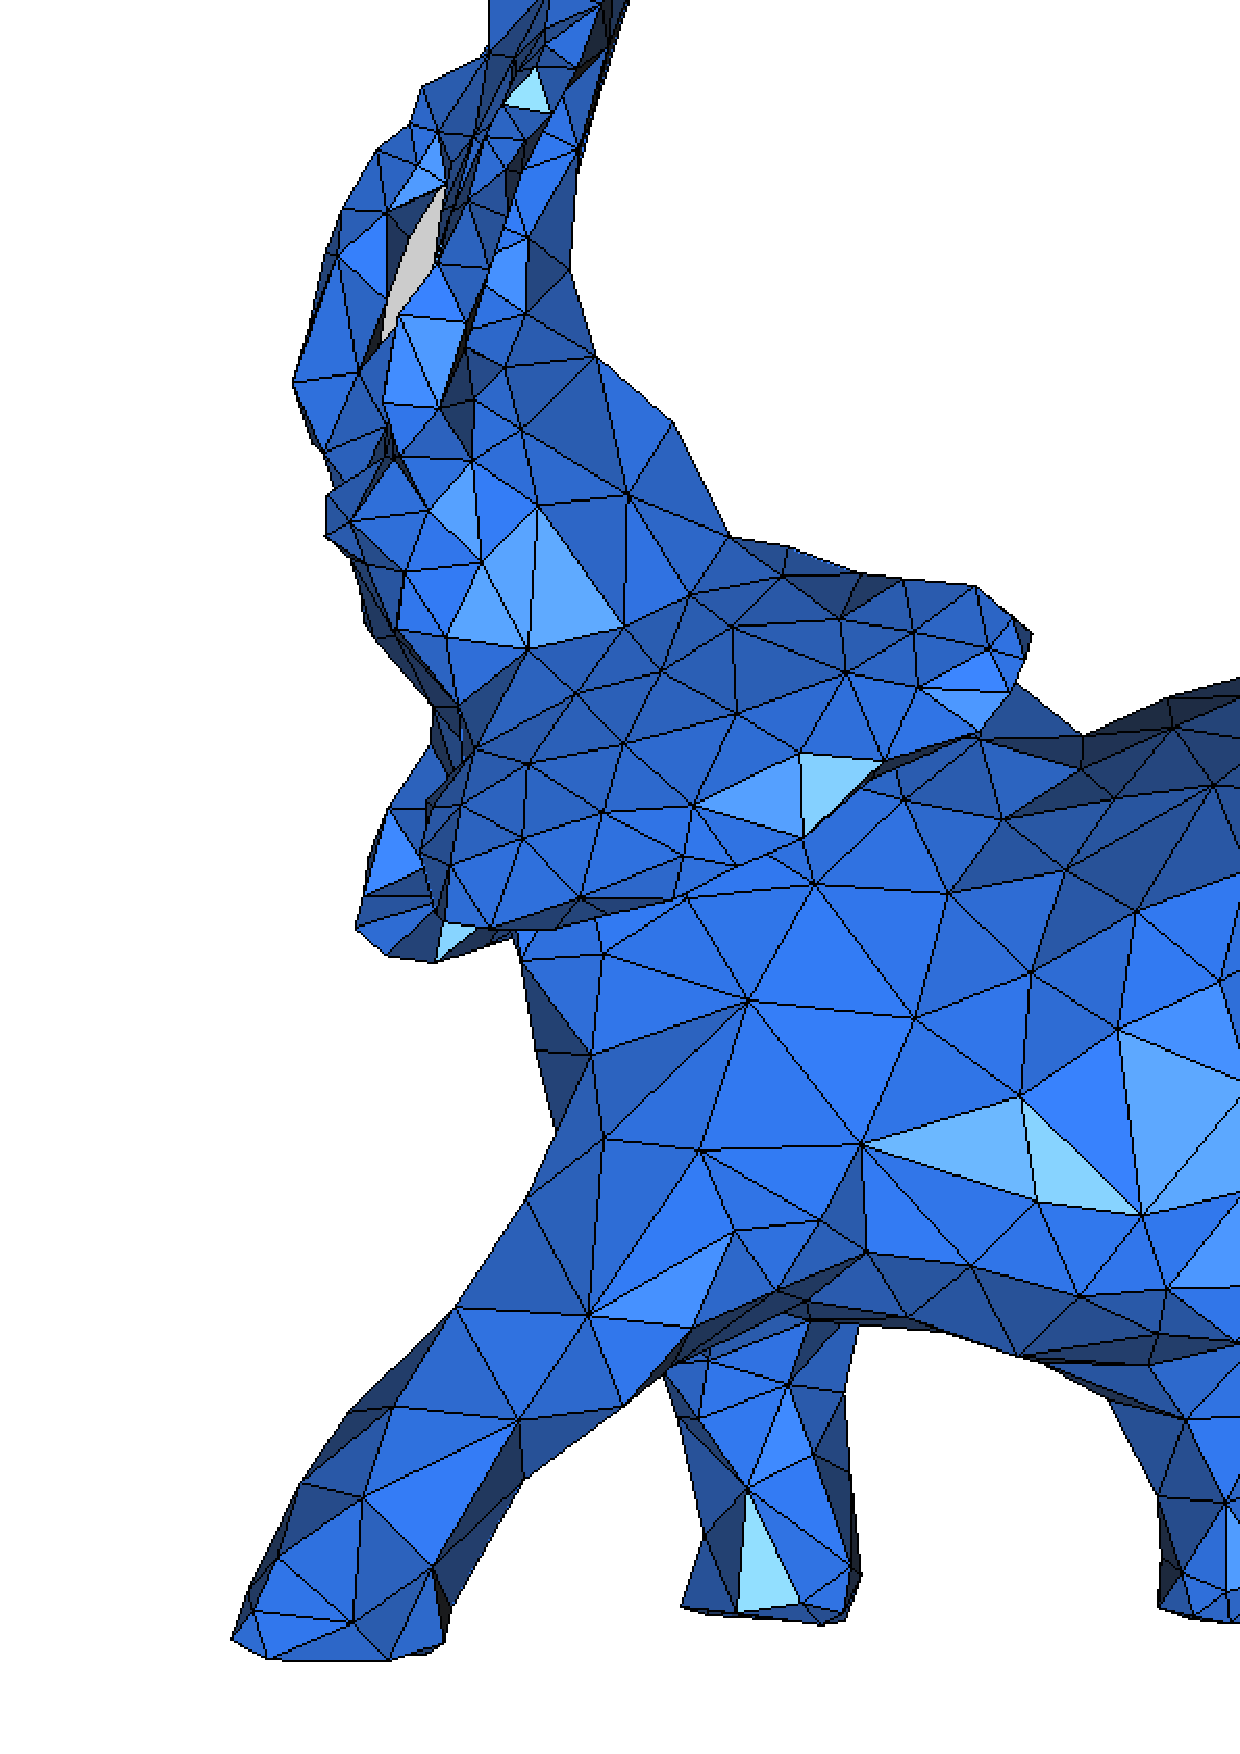
\includegraphics[height=7cm]{Mesh_3/pictures/polyhedral_domain}
   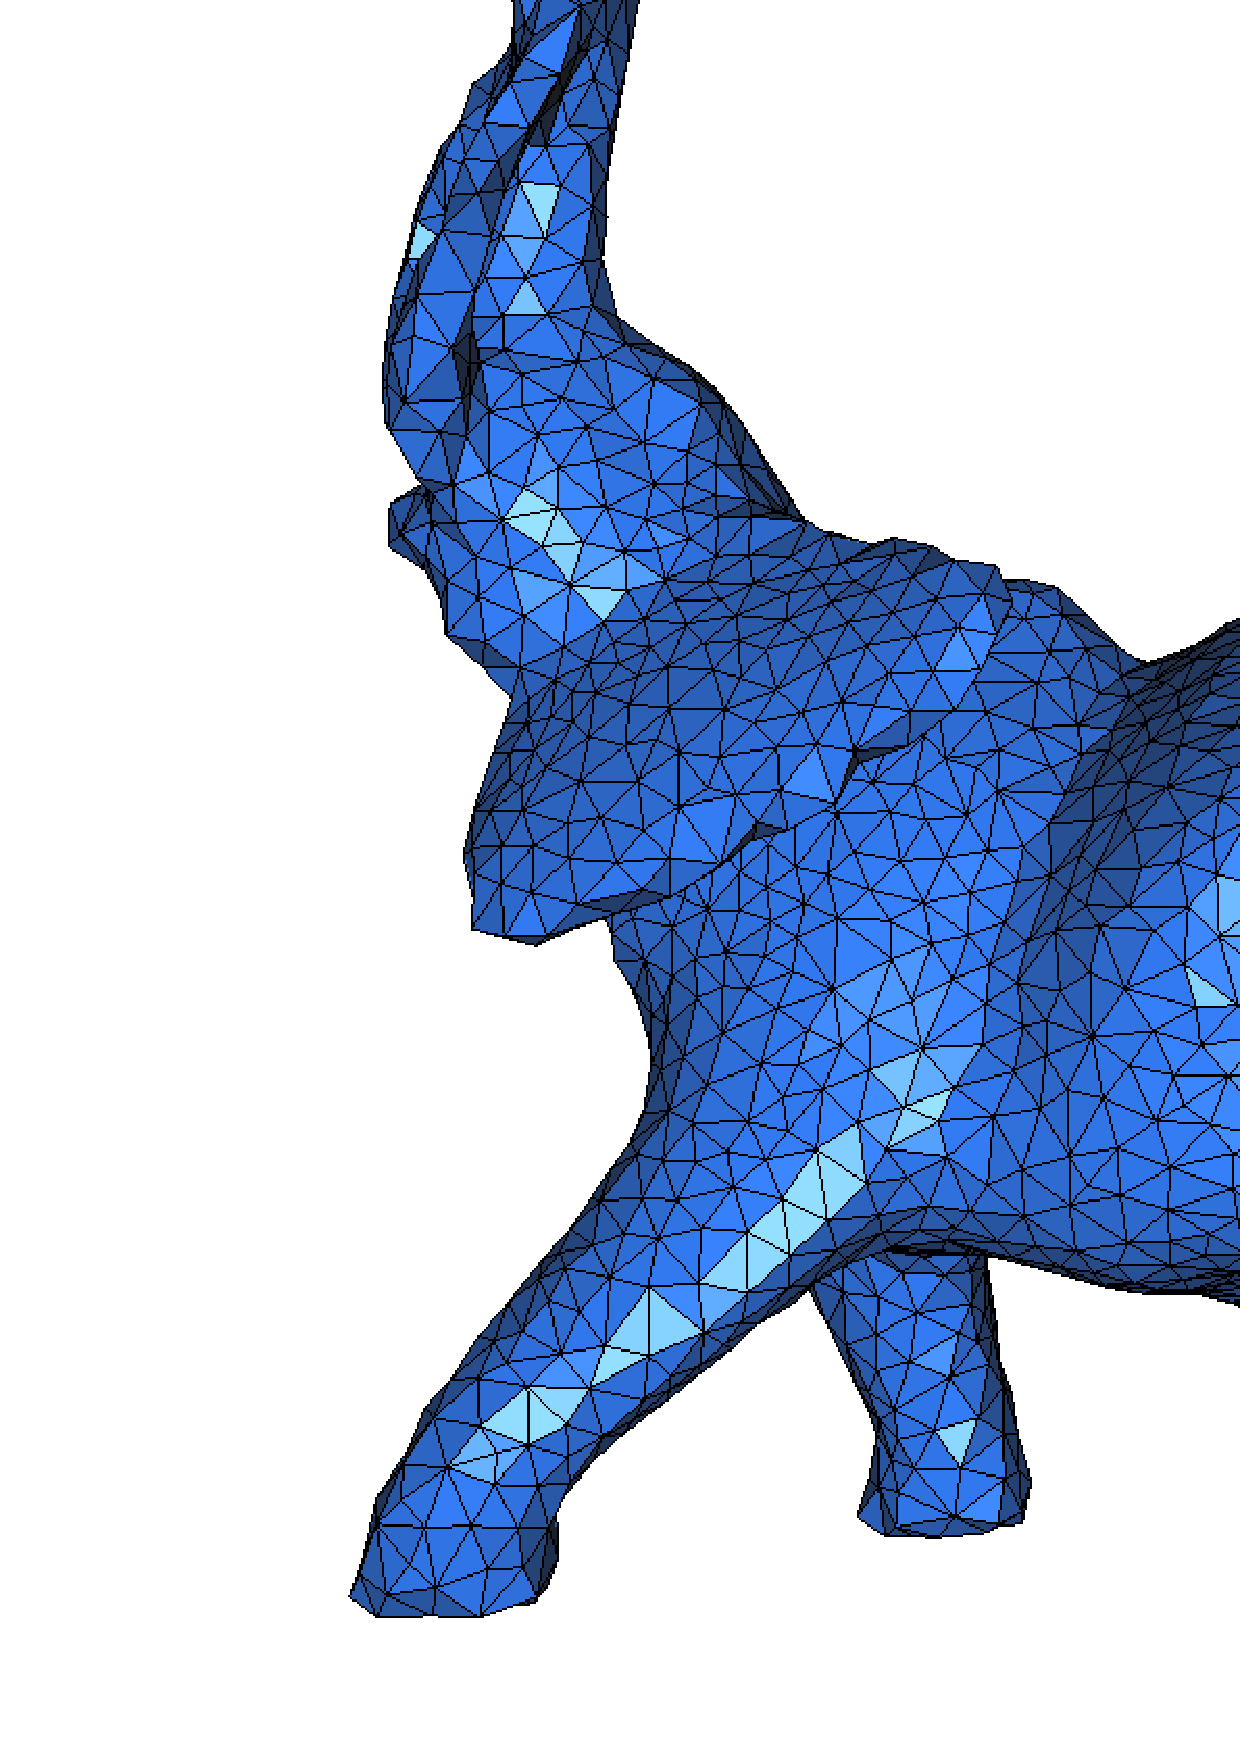
\includegraphics[height=7cm]{Mesh_3/pictures/polyhedral_domain_2}
 \end{ccTexOnly}
 \begin{ccHtmlOnly}
   <img border="0" src="./pictures/polyhedral_domain.jpg">
   <img border="0" src="./pictures/polyhedral_domain_2.jpg"><br/>
 \end{ccHtmlOnly}
 \caption{View of 3D meshes produced from a polyhedral domain. (i) 
   is a view of file out\_1.mesh and (ii) is a view of file
   out\_2.mesh. Code from
   subsection~\ref{Mesh_3_subsection_examples_polyhedral} generates
   these files.}
  \label{figure:polyhedral_domain}
\end{center}
\end{figure}


\subsection{Mesh Generation From a Segmented 3D Image}
\label{Mesh_3_subsection_examples_3d_image}
The following code produces  a 3D mesh from
a 3D image. The image is a segmented medical image  in which each 
voxel  is associated a label  in accordance with
the tissue  the voxel belongs to.
The domain is therefore a multi-domain
where each subdomain corresponds to a specific tissue.
The resulting mesh is shown in Figure~\ref{figure:liver_3d_image_mesh}.

\ccIncludeExampleCode{Mesh_3/mesh_3D_image.cpp}

\begin{figure}[ht]
\begin{center}
 \begin{ccTexOnly}
   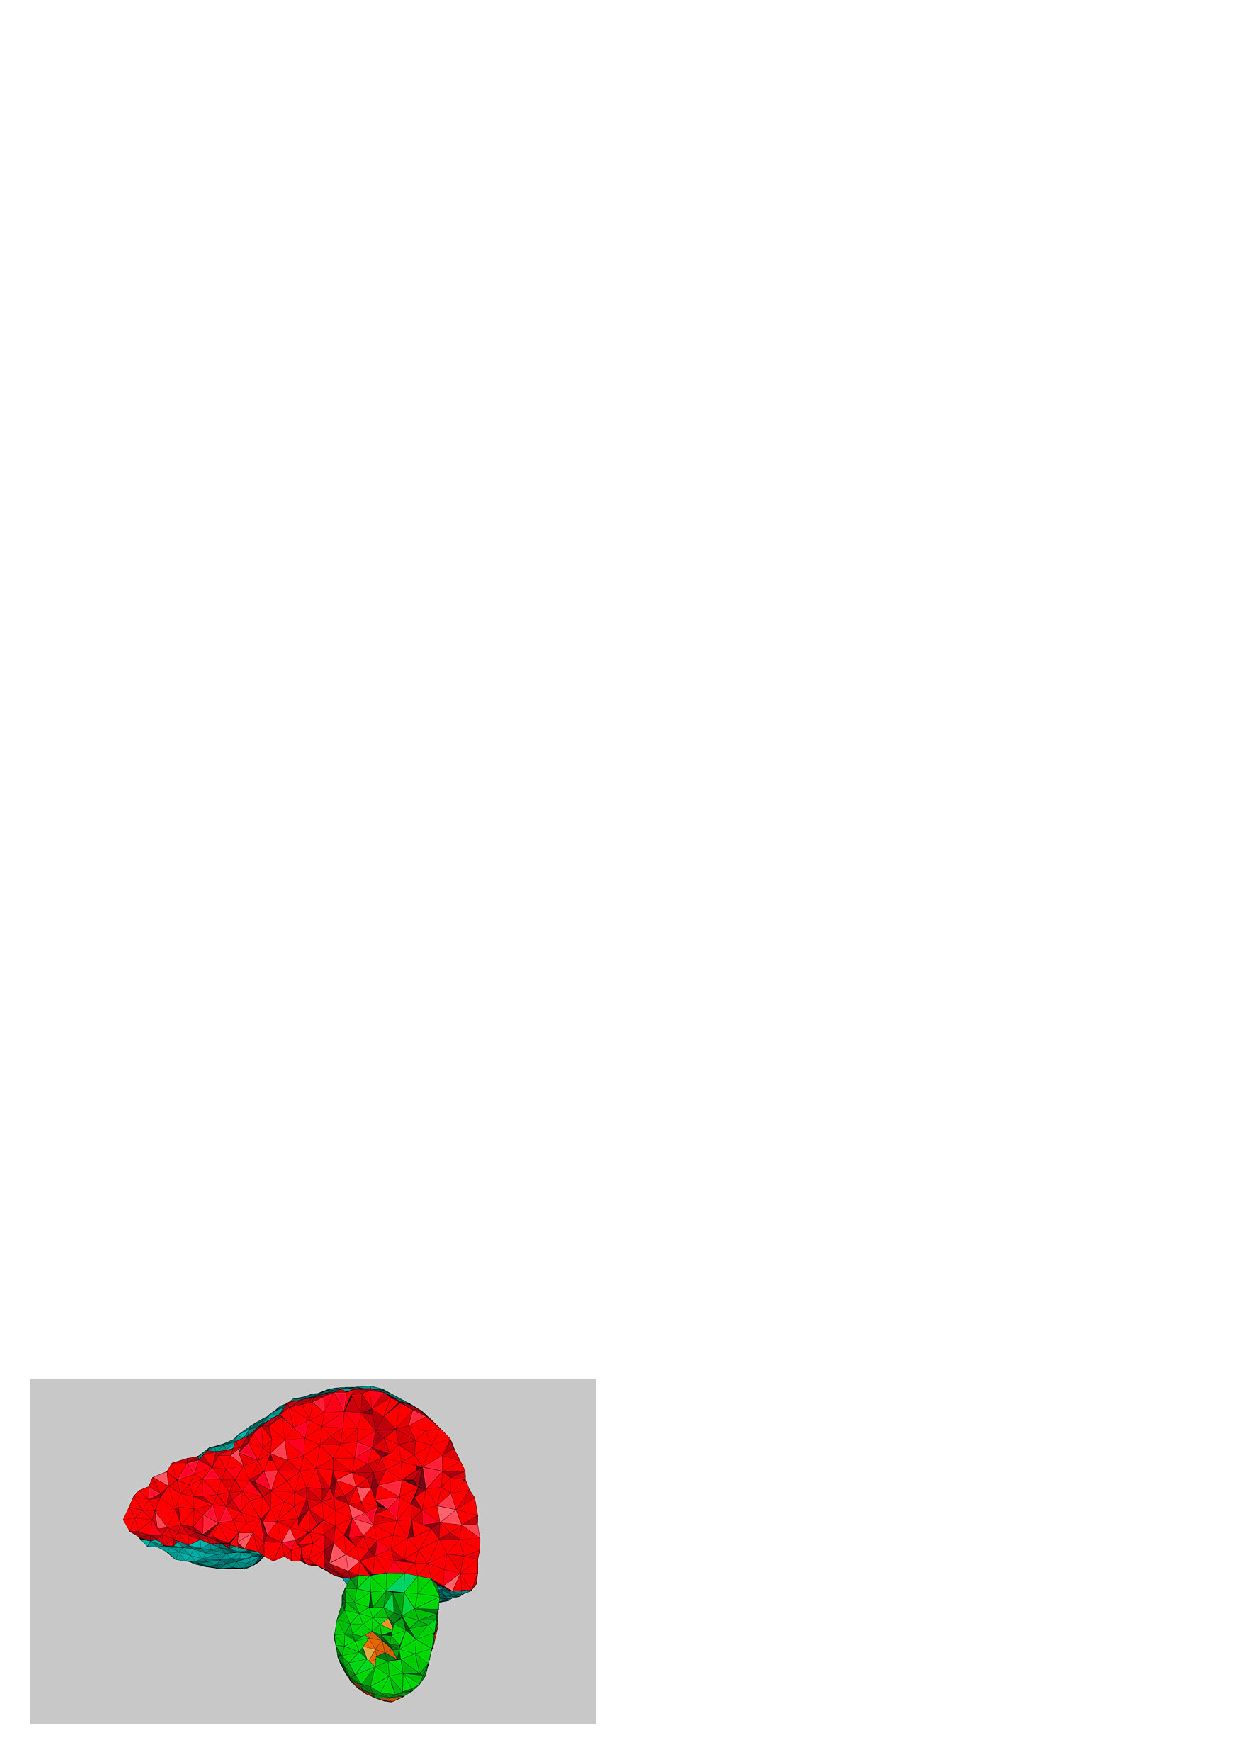
\includegraphics[width=14cm]{Mesh_3/pictures/liver}
 \end{ccTexOnly}
 \begin{ccHtmlOnly}
   <img border="0" src="./pictures/liver.jpg"><br/>
 \end{ccHtmlOnly}
 \caption{Cut-view of a 3D mesh produced from a segmented liver image. Code from
 subsection~\ref{Mesh_3_subsection_examples_3d_image} generates this file.}
  \label{figure:liver_3d_image_mesh}
\end{center}
\end{figure}
